\documentclass[12pt]{article}
%\documentclass{article}

\usepackage{times}
\usepackage[final]{graphicx}
\usepackage{hyperref}

\setlength{\topmargin}{-0.5in}
\setlength{\oddsidemargin}{0in}
\setlength{\evensidemargin}{0in}
\setlength{\textwidth}{6.5in}
\setlength{\textheight}{9.0in}

\begin{document}

\centerline{\bf \Large CS295/CS395/CSYS395: \href{CS295_395_Syllabus.pdf}{\underline{Evolutionary Robotics}}}

\vspace{0.5cm}

\centerline{\bf \large Programming Assignment 4 of 10}

\vspace{0.5cm}

\centerline{\large Assigned: Friday, September 23, 2011}

\vspace{0.5cm}

\centerline{\large Due: Friday, September 30, 2011 by midnight}

\vspace{0.5cm}

\noindent \textbf{Description:} In this assignment you will download, install and make some changes to Open Dynamics Engine (ODE), the open source physics engine we will be using for the remainder of this class. After installation and compilation, you will run a test application that comes with ODE which simulates a buggy (Fig. \ref{Fig}a). You will then change the radii of the wheels in the ODE code, re-compile and re-run the code to produce Fig. \ref{Fig}b. You will then comment out all the ODE code that creates, simulates and draws the objects and joints in this example program, producing the `empty world' shown in Fig. \ref{Fig}c. This will provide you with a blank canvas on which you will begin to build your robot in the next assignment. \\

\noindent \textbf{Important:} If you get stuck installing ODE, get on the ODE mailing list and ask your question; you will usually get a response in a couple of hours. \textbf{This means of course that you will have to start the assignment before the night before.} If you are still stuck, come see the instructor or teaching assistant.

\begin{enumerate}

\item \textbf{Back up your Python code from last week.} If you lose your laptop tomorrow, will you still have your code from assignments 1-3?

\item Download Open Dynamics Engine version 0.11.1. Download instructions can be found on ODE's
\href{http://ode.org/}{\underline{main page}}. Make sure to download from \href{http://sourceforge.net/projects/opende/files/}{\underline{Sourceforge}}.

\item Upzip the archive.

\item \textbf{If you are working on a Mac or on Linux}, follow the installation instructions found in INSTALL.txt. Once installed, skip to step 15.

\item \textbf{If you are working on Windows}, installing ODE is a bit trickier. Download and install the free C++ compiler
\href{http://www.softpedia.com/get/Programming/Other-Programming-Files/Microsoft-Visual-C-Toolkit.shtml}
{\underline{Visual C++ 2005 Express Edition}}. \textbf{Note from the T.A.:} There is a 2010 version of Visual C++ that is free from Microsoft. Visual Studio 2010 Express (includes C++).

\item Download and install \href{http://www.microsoft.com/downloads/en/details.aspx?FamilyId=0BAF2B35-C656-4969-ACE8-E4C0C0716ADB&displaylang=en}
{\underline{Windows Server 2003 Platform SDK}}. \textbf{Note from the T.A.:} There is an update to Windows Server 2003 Platform SDK which supports Windows 7, and earlier Windows versions including Vista and XP. Windows SDK for Windows 7 and .NET Framework 4


\item Open a Windows Command Prompt (in Windows XP, Start$\rightarrow$Run...$\rightarrow$cmd[enter]), and navigate to ode-0.11.1/build.

\item type \texttt{premake4 --with-demos --with-tests vs2005}

\item Close the Command Prompt and doubleclick on ode-0.11.1/build/vs2005/ode.sln, which will open ode, drawstuff (the drawing routines) and all of the demos in Visual C++.

\item in Visual C++ go to Tools/Options/Projects and Solutions/VC++ Directories.

\item Select `Show directories for'/Executable files, and add a directory pointer to \\
\texttt{C:/Program Files/Microsoft Visual Studio 8/VC/Microsoft Platform SDK for Windows Server 2003 R2/Bin}.

\textbf{Note from the T.A.:} VC++ Directories editing in Tools$\rightarrow$Options has been deprecated; directories are now available as a user property sheet that is added by default to all projects. Had to edit the output directory name in the linker property sheets for drawstuff and ode.

\item Select `Show directories for'/Include files, and add a directory pointer to \\
\texttt{C:/Program Files/Microsoft Visual Studio 8/VC/Microsoft Platform SDK for Windows Server 2003 R2/Include}

\item Select `Show directories for'/Library files, and add a directory pointer to \\
\texttt{C:/Program Files/Microsoft Visual Studio 8/VC/Microsoft Platform SDK for Windows Server 2003 R2/Lib}

\item Now Select Build/Build Solution to compile ODE, drawstuff and all the demo programs.

\item For windows users you should now find executables of the demo programs in \\ \texttt{ode-0.11.1/lib/debugdoubledll}. For Linux and Mac users you should find the executables in \texttt{ode-0.11.1/ode/demo}. Run the demo\_buggy executable.

\item You should see something like in Fig. \ref{Fig}a. Try driving the buggy up over the ramp, and get used to the mouse controls for moving the camera in ODE. Screencapture the simulation window, and paste the result into your document.

\item Open the code for demo\_buggy, and find the line that specifies the radii of the buggie's wheels. Multiply that variable by two, recompile, and re-run the demo. Screencapture the simulation window  (which should look like Fig. \ref{Fig}b) and paste the result into your document.

\item Re-open the code, and comment out all the code in the main function so that when you re-compile and re-run demo\_buggy, the program does not nothing, but does not crash.

\item Now you will allow the application to only create and destroy data structures, but not start the simulation. Uncomment the seven lines at the beginning of the the main function that define and set the \texttt{fn} data structure (\texttt{fn} controls drawing). Do not compile or run yet.

\item Uncomment the six lines following that create the world and the ground plane.

\item Uncomment the last four lines in the main loop (beside the \texttt{return 0} line) that destroy the world.

\item Re-compile, re-run and ensure that the program still starts and ends without crashing.

\item Now you will allow an `empty' simulation to run. Uncomment the line that starts the simulation:\\
\texttt{dsSimulationLoop (argc,argv,352,288,\&fn);}\\
This line creates a simulation window of 352x288 pixels and hands control to the simLoop function until the user stops the application.

\item Comment out all of the lines in the simLoop function. Recompile, re-run, and you should get an empty simulation as shown in Fig. \ref{Fig}c. Screencapture the window and copy it into your document.

\item Submit your document (containing three images) in .pdf format to the Teaching Assistant.

\end{enumerate}

\begin{figure}[!t]
\centerline{
a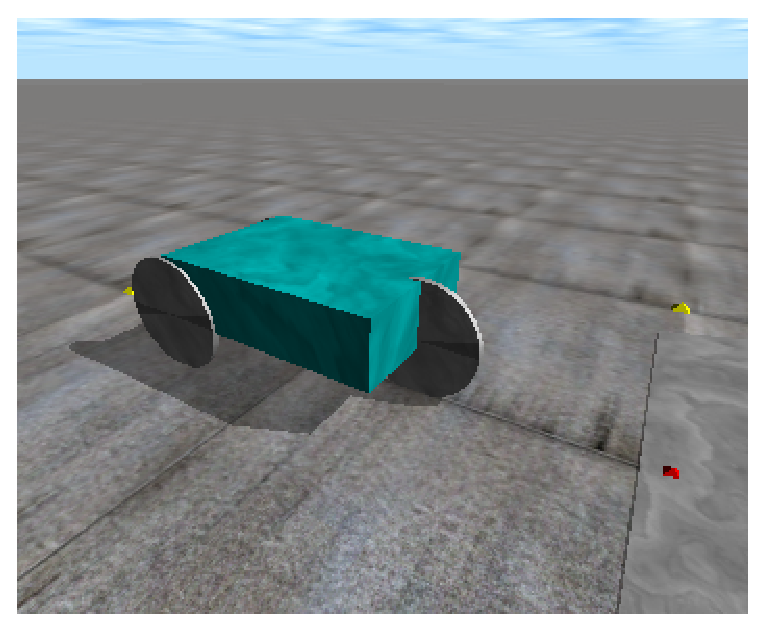
\includegraphics[width=0.48\textwidth]{Fig1a.eps}
b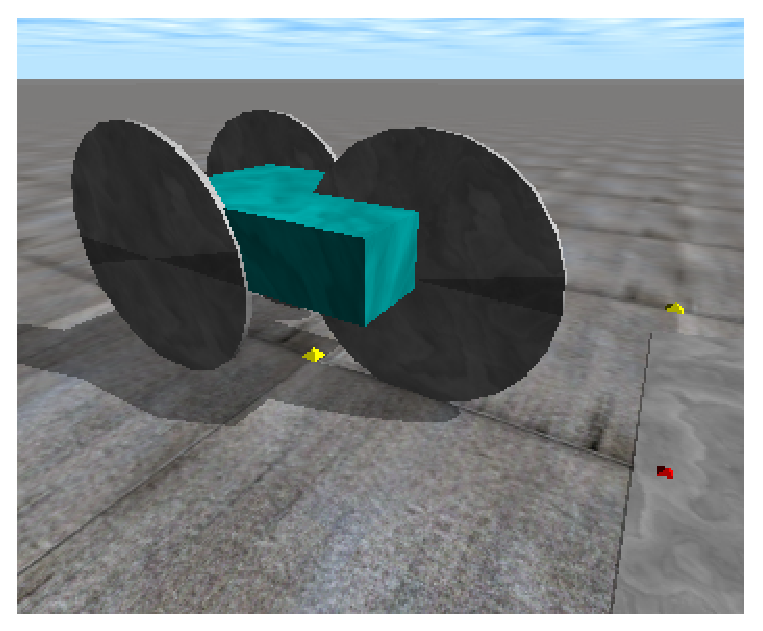
\includegraphics[width=0.48\textwidth]{Fig1b.eps}
}
\centerline{
c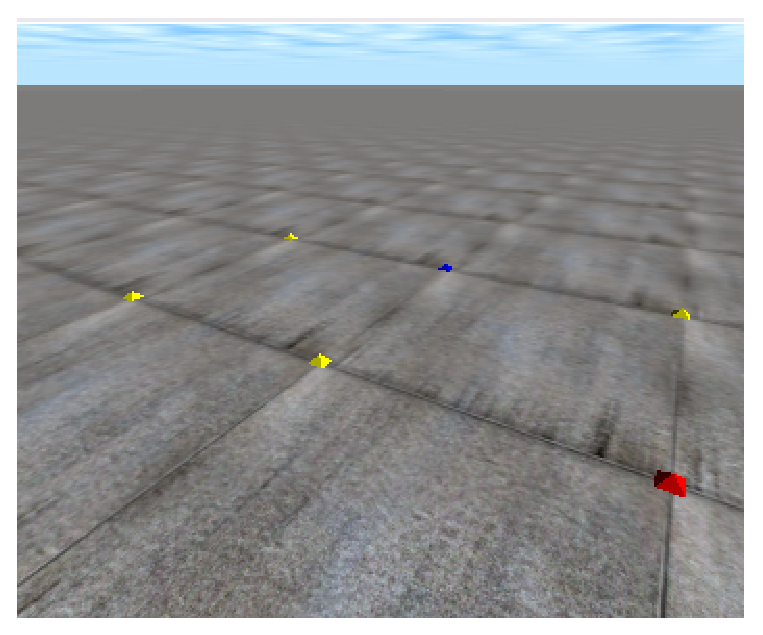
\includegraphics[width=0.48\textwidth]{Fig1c.eps}
}
\caption{
Successful compilation and execution of the test\_buggy program should produce \textbf{a}.
Changing the radii of the buggy's wheels should produce \textbf{b}.
Commenting out the construction, simulation and drawing of all objects and joints should produce \textbf{c}.}
\label{Fig}
\end{figure}

\end{document} 